\documentclass[preprint]{sigplanconf}

\usepackage{amsmath}
\usepackage{amssymb}
\usepackage{natbib}
\usepackage{multirow}
\usepackage{setspace}
\usepackage{balance}
\usepackage[all]{xy}

\newcommand{\backticks}[1]{\mathsf{\text{\textit{\`{}}}#1\!\text{\textit{\`{}}}}\;}

\include{paper}
%include paper.fmt
%format *> = "\mathbin{*\hspace{-5.8px}>}"
%format **> = "\mathbin{*\!*\hspace{-5.8px}>}"
%format *>> = "\mathbin{*\hspace{-5.8px}>\!\!>}"
%format ?> = "\mathbin{\raisebox{-.7px}{?}\hspace{-4px}>}"
%format ?== = "\mathbin{?\hspace{-4px}\equiv}"
%format `replaceExtension` = "\backticks{replaceExtension}"
%subst string a = "\!\text{\sf ``" a "\char34}\!"
%format context = "\Keyword{context}"
%format dependsS = "\Varid{depends\!^{*}}"
%format hashInclude = "\text{\sf ``\#include \textbackslash\char34\char34}"
%format Rule_m = "\Varid{Rule_m}"
%format Rule_s = "\Varid{Rule_s}"
%format build_m = "\Varid{build_m}"
%format build_s = "\Varid{build_s}"
%format Result_m = "\Varid{Result_m}"
%format Result_s = "\Varid{Result_s}"
%format skip_m = "\Varid{skip_m}"
%format skip_s = "\Varid{skip_s}"
%format <> = "\mathbin{\diamond}"

\hsdef{\begin{comment}
alpha,r,self,old
IO,Main,Development.Shake
Any,Eq,Show,Hashable,NFData,MonadIO,TypeRep
contents,target,rules
\end{comment}}

\begin{comment}
\h{.*}\begin{code}
import Data.Typeable
import Data.Hashable
import Control.DeepSeq
import Control.Monad.IO.Class
import Data.Monoid
import Control.Concurrent
import Data.Maybe
import Data.List hiding (find)
import Data.Binary
import Control.Monad
import System.Cmd
import System.Time
import qualified System.Directory
import System.Directory(copyFile,createDirectoryIfMissing)
data Map k v
data Set k
data Key
data Value
data Time = Time deriving (Ord,Eq)
type List_alpha a = [a]
hashInclude = "#include \""
ellipses = undefined
instance Binary ClockTime
instance NFData ClockTime
instance Eq Value
instance Typeable ClockTime
instance Hashable ClockTime
\end{code}
\h{.default}\begin{code}
instance Binary Dir
instance NFData Dir
instance Show Dir
instance Typeable Dir
instance Hashable Dir
instance Eq Dir
instance Binary File
instance NFData File
instance Show File
instance Typeable File
instance Hashable File
instance Eq File
instance Binary Files
instance NFData Files
instance Show Files
instance Typeable Files
instance Hashable Files
instance Eq Files
instance Binary FileTimes
instance NFData FileTimes
instance Show FileTimes
instance Typeable FileTimes
instance Hashable FileTimes
instance Eq FileTimes
writeFileLines :: FilePath -> [String] -> Action ()
shakeVersion :: ShakeOptions -> Int
system' :: String -> [String] -> Action ()
readFileLines :: FilePath -> Action [String]
(*>>) :: [FilePattern] -> ([FilePath] -> Action ()) -> Rules ()
writeFile' :: FilePath -> String -> Action ()
writeFileChanged :: FilePath -> String -> Action ()
cIncludes :: FilePath -> IO [FilePath]
systemOutput :: FilePath -> [String] -> Action (String, String)
data Status = Loaded | Missing | Error | Ready | Checking | Building
\end{code}
\h{.m}\begin{code}
(!) :: Set Rule_m -> Key -> Rule_m
data Rule
\end{code}
\h{.s}\begin{code}
(!) :: Set Rule_s -> Key -> Rule_s
\end{code}
\h{.s2}\begin{code}
instance Eq (Result_s -> Time)
instance Ord (Result_s -> Time)
\end{code}
\end{comment}


\newcommand{\file}{\textsf}
\newcommand{\prog}{\texttt}
\newcommand{\make}{\prog{make}}

\begin{document}
\conferenceinfo{ICFP'12,} {September 10--12, 2012, Copenhagen, Denmark.}
\CopyrightYear{2012}
\copyrightdata{978-1-60558-794-3/10/09}

\preprintfooter{}   % 'preprint' option specified.

\title{Shake Before Building}
\subtitle{Replacing Make with Haskell}

\authorinfo{Neil Mitchell}
           {\verb"ndmitchell@gmail.com"}

\maketitle

\begin{comment}
1. State the problem
2. Say why it�s an interesting problem
3. Say what your solution achieves
4. Say what follows from your solution
\end{comment}

\begin{abstract}
Most complex software projects are compiled using a build tool (e.g. \make{}), which runs commands in an order satisfying user-defined dependencies. Unfortunately, most build tools require all dependencies to be specified \textit{before} the build starts. This restriction makes many dependency patterns difficult to express, especially those involving files generated at build time. We show how to eliminate this restriction, allowing additional dependencies to be specified while building. We have implemented our ideas in the Haskell library Shake, and have used Shake to write a complex build system which compiles millions of lines of code.
\end{abstract}

\category{D.3}{Software}{Programming Languages}

\terms
Languages

\keywords
build-system, compilation, Haskell

\section{Introduction}
\label{sec:introduction}

A build tool, such as \make{} \cite{make}, takes a set of build rules, plus some input files, and produces some output files. Using \make{}, a build rule can be written as:

\ignore\begin{code}
{-"\textsf{result.tar : file1 file2}"-}
    {-"\textsf{tar -cf result.tar file1 file2}"-}
\end{code}

\noindent This rule says that the file \file{result.tar} depends on the inputs \file{file1} and \file{file2} (first line), and provides a command to build \file{result.tar} (second line). Whenever \file{file1} or \file{file2} change, the command will be run, and \file{result.tar} will be built.

But imagine we want to build \file{result.tar} from the list of files stored in \file{list.txt}. The dependencies of \file{result.tar} cannot be specified in advance, but depend on \textit{the contents} of \file{list.txt}. Unfortunately, the \make{} dependency system cannot express this pattern (for workarounds see \S\ref{sec:make_hacks}). Using the build tool we describe in this paper, we can write:

\h{expr}\begin{code}
"result.tar" *> \_ -> do
    need ["list.txt"]
    contents <- readFileLines "list.txt"
    need contents
    system' "tar" $ ["-cf","result.tar"] ++ contents
\end{code}

This rule describes how to build \file{result.tar}. We depend on (|need|) the file \file{list.txt}. We read each line from \file{list.txt} into the variable |contents| -- being a list of the files that should go into \file{result.tar}. Next, we depend on all the files in |contents|, and finally call the \prog{tar} program. If either \file{list.txt} changes, or any of the files listed by \file{list.txt} change, then \file{result.tar} will be rebuilt.

The key difference from \make{} (and nearly all other build tools) is that rather than specifying all dependencies \textit{in advance}, we allow further dependencies to be specified \textit{after} examining the results of previous dependencies. This difference is crucial to accurately describe many dependency relationships.

Consider the problem of dependencies stemming from files included by a C source file. Some build tools require these dependencies to be specified manually. Other build tools allow two separate phases, where dependencies are computed before the build starts. But if the build system generates C files and then compiles them, even a two phase system is insufficient, as the generated files are not available during the first phase. Our build tool has no such limitations -- it is able to easily handle generated files, even generated files which are only necessary due to being included by other generated files.

\subsection{Contributions}

We have implemented our build tool as a Haskell library, named Shake, which is available online\footnote{\url{http://hackage.haskell.org/package/shake}}. Shake provides a concise syntax for writing build systems (\S\ref{sec:user_view}), along with a high-performance implementation (\S\ref{sec:developer_view}). By implementing Shake as a Haskell library we allow rules to be written using the full power of Haskell, including the use of modules and functions to structure large build systems.

In addition to more flexible dependencies (\S\ref{sec:theory}), Shake also includes the important features of \make{}, such as minimal rebuilds (running only a subset of the rules when some subset of the inputs change, \S\ref{sec:cached_shake}), and parallelising the build (running multiple independent rules at the same time, \S\ref{sec:parallelism}). We allow rules to operate over any values, not limited to files, allowing us to track non-file dependencies (\S\ref{sec:directory_rule}) and properly handle commands producing multiple outputs (\S\ref{sec:multiple_outputs}). We have built a number of useful tools into Shake, including build rule checking (\S\ref{sec:lint}), profiling (\S\ref{sec:profiling}) and dependency analysis (\S\ref{sec:analysis}).

Various versions of Shake have been used at Standard Chartered for the past three years (\S\ref{sec:evaluation}). The build system creates over 30,000 build objects, with more than a million lines of source code and a million lines of generated code, in many programming languages. We originally implemented this build system using \make{}, but the result was slow to run, hard to maintain, and frequently caused spurious compile failures. Switching to Shake made our build system ten times shorter, made builds run twice as fast, and has solved our build system problems.

\section{Specifying Dependencies}
\label{sec:theory}

Most \make{}-like build tools start by constructing a graph from the dependency information, then traverse the graph, running the rules to build the required results (or use a topological sort, giving a similar effect). However, any approach based on a static dependency graph cannot permit additional dependencies to be specified while running the rules. As we saw in \S\ref{sec:introduction}, many examples \textit{require} additional dependencies to be specified while running the rules. The solution is simple -- we reject the idea that build tools should use a static dependency graph.

In this section we model the dependencies permitted by non-recursive \make{} \cite{miller:recursive_make}, along with our enhanced dependency scheme. We describe what it means for a build system to be correct, and how to support minimal rebuilds. In \S\ref{sec:user_view} and \S\ref{sec:developer_view} we show how to turn these ideas into a practical tool.

\subsection{Moving Dependency Specification}

While \make{} is heavily file and IO based, we choose to model the dependencies without these distractions. Our model uses the type |Key| for things that can be created or are dependencies (e.g. file names), and the type |Value| for the values associated with a |Key| (i.e.  file contents). With these types, we can define the main |build| function as:

\h{.m}\begin{code}
build :: Set Rule -> Key -> Value
\end{code}

The |build| function takes a (possibly infinite) set of rules and the target |Key| to build, and returns the |Value| associated with that |Key|. We restrict our model to building only one target, while \make{} allows multiple targets (i.e. a list of |Key|s to build). However, we can encode multiple targets by creating a distinguished key whose rule depends on the original targets and returns their values, and then use that key as the new target.

Using |build|, we can model \make{} with the |Rule| type:

\h{.m}\begin{code}
data  Rule_m = Rule_m
      {  creates  :: Key
      ,  depends  :: [Key]
      ,  action   :: [Value] -> Value
      }
\end{code}

A \make{} |Rule| (|Rule_m|) can be modelled as the |Key| it |creates|, the |Key|s it |depends| on, and the |action| that takes the depended upon |Value|s and produces the result |Value|. Note that all dependencies for a rule are specified \textit{before} running the action.

Using the same |build| function, we can model our enhanced dependency scheme as:

\h{.s .s2}\begin{code}
data  Rule_s = Rule_s
      {  creates  :: Key
      ,  action   :: Action
      }

data Action  =  Finished Value
             |  Depends Key (Value -> Action)
\end{code}

A Shake |Rule| (|Rule_s|) can be modelled as the |Key| it |creates|, and the |action| that creates the result. The |Action| either returns the |Finished| |Value|, or requires a new dependency with |Depends| -- specifying the |Key| it depends on, plus a function that takes the |Value| of that |Key| and produces a new |Action|.

The big difference from |Rule_m| is the introduction of dynamic dependencies. A rule can require additional dependencies, based on the values of previous dependencies. We can easily translate |Rule_m| to |Rule_s|, but the reverse is not possible -- |Rule_s| is strictly more powerful than |Rule_m|.

\subsection{Correctness}

Assuming a function which finds the |Rule| for a given |Key|, denoted by the operator |(!)|, we can write a function to build |Rule_m| targets as follows:

\h{.m}\begin{code}
build_m rules target = run (rules ! target)
    where run r = action r (map (build_m rules) (depends r))
\end{code}

Starting at the |target| |Key|, we find the associated |Rule_m|, run |build_m| on its dependencies, then run the |action|. A |Rule_m| build system is able to produce the result for a given |target| iff the expression \h{.m}|build_m rules target| is well-defined. If we assume all |action|s are total, then this expression is well-defined if you can build a finite dependency graph for the |target| with the available |rules|. This property can be checked without running any actions.

We can write a similar function to build |Rule_s| targets as follows:

\h{.s}\begin{code}
build_s rules target = run (action (rules ! target))
    where  run (Finished val) = val
           run (Depends dep act) = run (act (build_s rules dep))
\end{code}

Starting at the |target| |Key|, we find the |action| from the associated |Rule_s|, and run it. Once we reach |Finished| we are done; if we encounter a |Depends| we run |build_m| on that dependency before continuing. As before, a |Rule_s| build system is able to produce a result for a given |target| iff the expression \h{.s}|build_s rules target| is well-defined. However, unlike before, there is no obvious way to determine if the expression is well-defined in advance without detailed information about the |action| functions.

\subsection{Minimal Rebuilds}
\label{sec:minimal_rebuilds}

The build functions in the previous section may evaluate one rule many times during a single run, but real build systems should minimise the number of rules run. In a single build run, any rule should be run at most once -- a property that is easy to guarantee with a simple cache. Additionally, if a rule's dependencies have not changed since the last time it was run, the rule should not be rerun. In this section we describe how to avoid repeating |Rule_m| rules whose dependencies have not changed, enhancing the scheme followed by \make{}, then apply the same ideas to |Rule_s|.

\subsubsection{Minimal Rebuilds with |Rule_m|}
\label{sec:cached_make}

To avoid repeating rules whose dependencies have not changed, \make{} does not run any rules where the dependent files have older modification times than the result file. We use a similar scheme, adapted for arbitrary |Key|/|Value| types. Whenever a rule is run, we create a |Result_m|:

\h{.m}\begin{code}
data Result_m = Result_m
    {  created  :: Key
    ,  result   :: Value
    ,  built    :: Time
    }
\end{code}

|Result_m| contains the |Key| the rule |created|, the |result| |Value|, and the |Time| when the result was |built|. We store all |Result_m| values between build runs using a database, and skip rerunning a |Rule_m| if the result was built more recently than its dependencies. In common with \make{}, we assume the rules do not change between runs (see \S\ref{sec:changing_rules} for workarounds). To determine if we should skip, we require the result for this rule's key from the previous build run (named |old|) and a way to demand results for this build run (named |ask|):

\h{.m}\begin{code}
skip_m :: Result_m -> (Key -> Result_m) -> Rule_m -> Bool
skip_m old ask r = all ((<= built old) . built . ask) (depends r)
\end{code}

The |skip_m| function returns |True| if a rule does not need running. We require the results for all dependencies, then check that they were built before this rule was last run.

The \make{} approach of relying on modification times can fail if the system clock changes, if the clock resolution is too coarse, or if a file has its modification time set to a time in the past (such as when extracting a backup). Therefore, instead of using the system time for |built|, we use the number of runs of this build system, incrementing |Time| each run. This approach guarantees that |Time| is monotonically increasing.

A convenient property of \make{} is that no additional data need be stored between runs, since the file system already stores modification times. In contrast, we must store the |Time| and |Result_m| values in a database (interestingly, an additional data store is required for many advanced build systems, see \S\ref{sec:related_work}). However, for some types of rules, such as when |Key|s are filenames and |Value|s are modification times, the |Value|s are stored in both the |Result_m| database \textit{and} the file system. If an inconsistency is detected, we must discard our stored |Result_m|. To detect inconsistencies, we require the following function:

\begin{code}
validStored :: Key -> Value -> Bool
\end{code}

This function should return |True| if the |Key|'s |Value| is not stored elsewhere, or if it is stored but the |Value| is consistent. As an example for files, |validStored| should return |True| only if the file exists, and has the same modification time.

\subsubsection{Minimal Rebuilds with |Rule_s|}
\label{sec:cached_shake}

To achieve minimal rebuilds with |Rule_m| we rely on having the dependencies available without executing the action, something that is not available with |Rule_s|. To solve this problem, we include the list of dependencies in |Result_s|, and use them in |skip_s|:

\h{.s}\begin{code}
data Result_s = Result_s
    {  created :: Key, result :: Value, built :: Time
    ,  depends :: [Key]
    }

skip_s old ask r = all ((<= built old) . built . ask) (depends old)
\end{code}

Compared to |skip_m|, we have made one small change -- instead of using \h{.s}|depends r|, we use \h{.s}|depends old|. For the stored |depends| to be valid we rely on the rule's |action| not changing, and that the |action| is pure (see \S\ref{sec:lint} for necessary restrictions when we allow IO actions). With this modification we are able to ensure minimal rebuilds using |Rule_s|. We still require the |validStored| check from the previous section.

\subsubsection{Unchanging Results}
\label{sec:unchanging_results}

The \make{} tool has a requirement that a rule action \textit{must} modify the file it creates, otherwise the rule will be repeatedly rerun, as the result will remain older than its dependencies. This requirement stems from using the modification time as both the |result| and the |built| time, but since we store these fields separately, we can eliminate some unnecessary rebuilds.

Instead of storing just the |built| time, we also store the |changed| time -- when the |result| last changed. Whenever we create a result we use the current time for |built|, but if the |result| |Value| is the same as last time, we use the previous |changed| time. We can rewrite |skip_s| to take advantage of this additional information:

\h{.s2}\begin{code}
data Result_s = Result_s
    {  created :: Key, result :: Value, built :: Time, depends :: [Key]
    ,  changed :: Time
    }

skip_s old ask r =
    all ((<= built old) . changed . ask) (depends old)
\end{code}

We have made one small change -- instead of checking against the |built| time of the dependencies, we check against their |changed| time. It is important to still compare against \h{.s2}|built old| because running a rule may not update its |changed| time, but will always update its |built| time, thus we avoid rebuilding repeatedly when the result does not change. Since it is always the case that \h{.s2}|changed <= built|, |skip_s| will now return |True| more often.

In some situations, support for unchanging results can reduce rebuild times from many minutes to seconds. As an example, consider a file generated by the build system. If the generator changes it is necessary to regenerate the file, but there is a chance the result will not have changed. By supporting unchanging files we can avoid rebuilding everything depending on that file.

\section{Shake in Haskell}
\label{sec:user_view}

In this section we use the theory from \S\ref{sec:theory} to create a practical build tool, implemented as a Haskell library. In particular, we describe how to replace |Key| and |Value| with polymorphism, how to integrate IO actions and how to define a set of rules. We present the developer interface to Shake, but leave most implementation concerns to \S\ref{sec:developer_view}.

\subsection{A Shake Example}
\label{sec:c_example}

\begin{figure}
\begin{code}
{-"\Keyword{import}\;\Conid{Development.Shake}"-}
import System.FilePath

main = shake shakeOptions $ do
    want ["Main"]

    "Main" *> \out -> do
        cs <- getDirectoryFiles "." "*.c"
        let os = map (++ ".o") cs
        need os
        system' "gcc" $ ["-o",out] ++ os

    "*.c.o" *> \out -> do
        let c = dropExtension out
        need [c]
        headers <- cIncludes c
        need headers
        system' "gcc" ["-o",out,"-c",c]

cIncludes :: FilePath -> Action [FilePath]
cIncludes x = do
    (stdout,_) <- systemOutput "gcc" ["-MM",x]
    return $ drop 2 $ words stdout
\end{code}
\caption{A Shake build system for C code.}
\label{fig:demo}
\end{figure}

Figure \ref{fig:demo} shows an example build system in Shake. Running this program will build \file{Main} from all the \file{*.c} files in the current directory. If we add or remove a \file{.c} file, or change any of the \file{.c} files or the header files they @#include@, then the necessary files will be rebuilt.

The build system produces (|want|s) the file \file{Main}. To generate \file{Main} we list all the C files in the current directory, add the extension \file{.o} (object files), require those files to be built (|need| them), then call \prog{gcc} to link them. To build an object file we take the associated C file and call the function |cIncludes| to get the headers it requires. We |need| those headers, then call \prog{gcc} to do the compilation. The |cIncludes| function works by calling \prog{gcc -MM}, causing \prog{gcc} to generate the dependency information on the standard output.

This example demonstrates a number of features of Shake based build systems:

\begin{description}
\item[It's Haskell] The |main| entry point can call |shake| directly, but it can also do command line processing (\S\ref{sec:command_line}), or anything else. We have defined a local function, |cIncludes|, helping to split the build system into components that can be reused. We make use of the existing \ignore|filepath| library.
\item[Expressive dependencies] The call to |getDirectoryFiles| is tracked (\S\ref{sec:directory_rule}) -- adding or removing files will trigger a rebuild. We track the dependencies introduced by @#include@ directives.
\item[We use system commands] We use \prog{gcc} to compile, to link, and to determine the headers required by the C files. We can freely use both Haskell functions and system commands to generate build results.
\end{description}

As a practical concern, for many larger projects there are often multiple compilers that produce object files with the \file{.o} extension. We solve this problem by making the C compiler use the extension \file{.c.o}, the Haskell compiler use \file{.hs.o} etc, allowing different rules for each type of object.

\subsection{Core Shake}
\label{sec:core_shake}

\begin{figure}
\begin{code}
data  ShakeOptions = ShakeOptions
      {  shakeFiles    :: FilePath
      ,  shakeThreads  :: Int
      {-" ,  \ldots"-}
      }
shakeOptions = ellipses -- default set of options

data Rules alpha
instance Monad Rules
instance Monoid alpha => Monoid (Rules alpha)

data Action alpha
instance Monad Action
instance MonadIO Action

class (
    Typeable  key, Typeable  value,
    Binary    key, Binary    value,
    Eq        key, Eq        value,
    Hashable  key, Hashable  value,
    Show      key, Show      value,
    NFData    key, NFData    value
    ) => Rule key value where
    validStored :: key -> value -> IO Bool

run :: ShakeOptions -> Rules () -> IO ()

action :: Action () -> Rules ()

rule, defaultRule :: Rule key value =>
    (key -> Maybe (Action value)) -> Rules ()

apply   :: Rule key value =>  [  key]  -> Action [  value]
apply1  :: Rule key value =>     key   -> Action    value
\end{code}
\caption{Primitive operations in Shake}
\label{fig:shake_core}
\end{figure}

The core interface to Shake is given in Figure \ref{fig:shake_core} -- everything else is defined on top. At its essence, a Shake build system is a set of rules. We can run the rules with |run|, create new rules with |rule|/|defaultRule|, and when defining a rule we can express dependencies with |apply|/|apply1|.

We execute a set of rules using the |run| function, which also takes an options record. Typical options include which file to use for the database (|shakeFiles|) and the number of processors to use (|shakeThreads|).

Every |key|/|value| rule pair used in Shake must be a member of the |Rule| class. The |Rule| class defines the method |validStored| to determine whether a value is consistent with any value stored externally (\S\ref{sec:minimal_rebuilds}). Each |key| and |value| type must also be a member of several type classes:

\begin{description}
\item [Typeable] We allow multiple types of rules in a single build system. To distinguish the types, we require a |Typeable| constraint, allowing us to obtain an explicit |TypeRep| \cite{lammel:syb}.
\item [Binary] We require |Binary| serialisation, allowing us to store the results between runs, to achieve minimal rebuilds (\S\ref{sec:minimal_rebuilds}).
\item [Eq] We require equality to look up results for |key|s and to test if |value|s have changed (\S\ref{sec:unchanging_results}).
\item [Hashable] We require |Hashable| to accelerate looking up results for |key|s. The |Hashable| requirement for |value| is currently unused, but is included for consistency.
\item [Show] We require |Show| for debugging messages, profiling and analysis (\S\ref{sec:handling_errors}, \S\ref{sec:profiling}).
\item [NFData] We require |NFData| to ensure that values are fully evaluated when they are computed, ensuring errors occur in a timely manner (\S\ref{sec:handling_errors}).
\end{description}

Most rules are defined with |rule|, whose argument is a function which takes a single |key| value, and returns |Nothing| to indicate that this rule does not build this |key|, or |Just| with the action that builds the associated |value|. Compared to the theory from \S\ref{sec:theory}, |rule| can be thought of as defining a rule template, which matches a potentially infinite number of |key|s, allowing us to represent an infinite number of rules with a finite number of calls to |rule|. The function |defaultRule| allows a rule to be defined with a lower priority, which is used if no |rule|s match (see \S\ref{sec:file_rules}). If two rules of the same priority match the same key then an error is raised. Instead of defining targets to build, we use |action| to specify actions that are always run, which typically call |apply|.

The |Rules| type is a commutative |Monoid|, allowing two sets of rules to be joined to produce a new set of |Rules|. In practice, the syntactic sugar supported by |Monad| offers a very natural way to define rules, allowing a set of rules to be introduced with |do| and then simply written below each other. To support a |Monad| instance for |Rules| we add an additional type parameter |alpha| (almost always instantiated to |()|) and make |(>>)| join two sets of rules.

To define actions we use the |Action| type, which has a |Monad| instance to allow actions to be executed sequentially. The |Action| type has an instance for |MonadIO|, allowing users to call arbitrary |IO| functions using |liftIO| to translate \h{type}|IO alpha| to \h{type}|Action alpha|. Dependencies can be expressed using the function |apply1| which takes a |key|, ensures the |key| is built, and returns the associated |value|. The |apply| function can be thought of as |mapM apply1|, but may build the necessary |key|s in parallel (\S\ref{sec:parallelism}).

\subsection{Wildcard File Patterns}
\label{sec:file_pattern}

The \make{} tool supports the syntax \textsf{\%.c} to match any files ending with \file{.c}. We define a similar notation, allowing |"*"| to match any part of a filename and |"//"| to match any number of directories, using the definitions:

\begin{code}
type FilePattern = String
(?==) :: FilePattern -> FilePath -> Bool
\end{code}

As an example, |"*.c" ?== "foo.c"| returns |True|, while |"*.c" ?== "foo.h"| returns |False|. We reuse the |FilePattern| type in several of our rules.

\subsection{Defining Rule Types}
\label{sec:directory_rule}

\begin{figure}
\begin{code}
import qualified System.Directory as IO

data Dir = Dir FilePath FilePattern
-- plus all necessary instances

go :: Dir -> IO [FilePath]
go (Dir dir pat) =
    liftM (filter (pat ?==)) $ IO.getDirectoryContents dir

instance Rule Dir [FilePath] where
    validStored q a = liftM (== a) $ go q

getDirectoryFiles :: FilePath -> FilePattern -> Action [FilePath]
getDirectoryFiles dir pat = apply1 $ Dir dir pat

defaultDir :: Rules ()
defaultDir = defaultRule $ Just . liftIO . go
\end{code}
\caption{Implementation of |getDirectoryFiles|.}
\label{fig:getdirectoryfiles}
\end{figure}

A typical Shake build system will use a handful of different |Rule| instances, usually all provided by the Shake library. To aid end users, we suggest that people defining rule types also define sugar functions, as we have done for the rule types included with Shake. As an example of defining a rule type, we give the code for |getDirectoryFiles| in Figure \ref{fig:getdirectoryfiles}. This function takes a directory, and a file pattern (\S\ref{sec:file_pattern}), and returns the list of files that match.

We start by defining a |key| data type (|Dir|), along with a function that computes the result (|go|). We define a |Rule| instance mapping from the |Dir| data type to the result type of \h{type}|[FilePath]|, which uses equality to check if a previous result is still valid. We define |getDirectoryFiles| as a strongly typed wrapper around |apply1|, and |defaultDir| as a wrapper around |defaultRule|. Anyone using |getDirectoryFiles| must include |defaultDir| in their rule set, so the |defaultRule| for |Dir| is available. We do not export the |Dir| constructor, forcing people to use the wrappers.

\subsection{File Based Rules}
\label{sec:file_rules}

\begin{figure}
\begin{code}
import qualified System.Directory as IO

newtype File = File FilePath
-- plus all necessary instances

getFileTime :: FilePath -> IO (Maybe ClockTime)
getFileTime x = do
    b <- IO.doesFileExist x
    if not b then return Nothing else
        liftM Just $ IO.getModificationTime x

instance Rule File ClockTime where
    validStored (File x) t = fmap (== Just t) $ getFileTime x

need :: [FilePath] -> Action ()
need xs = do
    apply $ map File xs :: Action [ClockTime]
    return ()

want :: [FilePath] -> Rules ()
want xs = action $ need xs

defaultFile :: Rules ()
defaultFile = defaultRule $ \(File x) -> Just $ do
    res <- liftIO $ getFileTime x
    let msg = "Error, file does not exist and no rule: " ++ x
    return $ fromMaybe (error msg) res

(?>) :: (FilePath -> Bool) -> (FilePath -> Action ()) -> Rules ()
(?>) test act = rule $ \(File x) ->
    if not $ test x then Nothing else Just $ do
        liftIO $ createDirectoryIfMissing True $ takeDirectory x
        act x
        res <- liftIO $ getFileTime x
        let msg = "Error, rule failed to build the file: " ++ x
        return $ fromMaybe (error msg) res

(**>) :: [FilePattern] -> (FilePath -> Action ()) -> Rules ()
(**>) test act = (\x -> any (?== x) test) ?> act

(*>) :: FilePattern -> (FilePath -> Action ()) -> Rules ()
(*>) test act = (test ?==) ?> act
\end{code}
\caption{Implementation of file rules.}
\label{fig:file_rules}
\end{figure}

While our build system is not restricted to rules dealing with files, in practice many build systems are file orientated. When implementing file rules, the filename is an obvious |key|, but |value| could be either modification time or a hash of the file contents (e.g. SHA1). In practice, we found that using modification time is faster (significantly faster for large files) and being able to force rebuilds using the \prog{touch} command is highly convenient when writing build rules. Of course, our design allows anyone to define a new type of file rule, based on file content hashes.

We define file rules in Figure \ref{fig:file_rules}. To force files to be built, we define |need| and |want|. The |need| action adds a dependency on all the modification times of the files, and is typically used before performing some IO action that uses the files. We define |want| to specify targets, implemented as |need| run by |action|.

We define |defaultFile| as a rule that checks if the file already exists, and if so uses it. Source files will have no associated rules to build them, so this rule just records their modification time. If a file has no rules (since any rules would be run in preference to the default rule), and does not exist, we raise an error. As with |defaultDir|, anyone using |want|/|need| should include |defaultFile| in their rule set.

We define new file rules using |(?>)|, which takes a predicate to match against the file name and an action to run. This function ensures the correct |key|/|value| types, and obtains the modification time afterwards. Before running the action we create the directory containing the output file, an idea taken from the Ninja build system \cite{ninja}. We found that when running a large set of newly written rules, often one rule would create the output directory while another did not -- meaning some rule execution orderings worked while others failed. Automatically creating the output directory removes this source of failure.

While |(?>)| is the ultimate file creation rule, we define two additional operators, using the file wildcard match operator |(?==)| from \S\ref{sec:file_pattern}. We define |(*>)| for matching a single pattern, for example |"*.c" *> ellipses|, in a similar style to \make{}. We define |(**>)| for matching any one of a set of patterns.

\subsection{Automatically Include Default Rules}
\label{sec:include_default_rules}

With the rule types already defined, users can write a build system using Shake. Unfortunately, if the user forgets to include the |defaultFile| rule, there is likely to be a runtime error. Instead of requiring the user to remember to include the default rules, we define a wrapper function |shake| which includes all the standard default rules:

\begin{code}
shake opts rules = run opts $ do
    defaultDir   -- \S\ref{sec:directory_rule}
    defaultFile  -- \S\ref{sec:file_rules}
    ellipses
    rules
\end{code}

In addition to the directory and file rules, we also include rules that query the existence of files, always force a rule to rerun, store arbitrary configuration data in a tracked manner and build multiple files in one action. All these rules are defined similarly to the directory and file rules.

The astute reader may be wondering why we can't specify default rules as an additional member in the |Rule| type class, allowing the default rule to be found from the type, and avoiding the need for the |shake| wrapper around |run|. Alas, that solution doesn't work because we need explicit rules of each type to deserialise dynamically typed values (for full details see \S\ref{sec:dynamically_typed}).

\subsection{Additional Functions}
\label{sec:derived}

The IO function |readFile| is only safe if the file being read has previously had |need| called on it, tracking the dependency (for more IO safety properties see \S\ref{sec:lint}). To help build system authors, we define a safe wrapper, |readFile'|, which includes the call to |need|:

\begin{code}
readFile' :: FilePath -> Action String
readFile' x = need [x] >> liftIO (readFile x)
\end{code}

We also define |readFileLines| which is like |readFile'|, but splits the contents of the file into lines (therefore the first |need| call in the example from \S\ref{sec:introduction} is unnecessary, but not harmful, as |readFileLines| will also call |need|). We define |writeFileLines| for writing files containing a list of lines. The function |writeFileChanged| writes a file, but only if the contents have changed, avoiding some rebuilds due to unchanging results (\S\ref{sec:unchanging_results}).

We define the |system'| function which runs a system command, but fails if the exit code represents failure, and also records profiling information (see \S\ref{sec:profiling}). The |system'| function should be used carefully, as it cannot tell which files the system command may depend on, so explicit |need| commands must be used. We recommend writing wrappers around system commands which insert the appropriate |need| calls (see \S\ref{sec:lint} for which |need| calls are required).


\section{Implementing Shake}
\label{sec:developer_view}

We have implemented Shake, and used it extensively. In this section we sketch some of the main implementation challenges and how they can be overcome. We first describe how to handle different |key|/|value| types within a single build system, then how to deal with errors, and finally how to execute the rules efficiently and with maximum parallelism. Readers interested in more details are encouraged to download the full implementation (see \S\ref{sec:introduction}).

\subsection{Dynamically Typed Values}
\label{sec:dynamically_typed}

A single Shake program can use multiple types for keys and values. To work with heterogenous values in Haskell we define:

\ignore\begin{code}
data Any = Any (forall alpha bullet
    (  Typeable alpha, Binary alpha, Eq alpha
    ,  Hashable alpha, Show alpha, NFData alpha) => alpha)
\end{code}

This definition, using existentials \cite{laufer:existentials}, allows any type supporting all the required type classes to be stored as type |Any|. We define |Key| and |Value| as synonyms for |Any|. We can implement |Eq|, |Hashable|, |Show| and |NFData| instances for |Any| without difficulty, often by appealing to the |TypeRep| provided by the |Typeable| instance.

Implementing a |Binary| instance for |Any| is harder. Serialising a value is easy, we serialise the |TypeRep| followed by the value. However, deserialising is problematic -- we can deserialise the |TypeRep|, but to deserialise the value we need to obtain the |Binary| instance for that type. Our solution is to keep a mapping from |TypeRep| to |Any|, and after deserialising the |TypeRep| find the associated |Any| and use that |Binary| instance. As a consequence, we cannot deserialise any file containing a |TypeRep| not present in our mapping. We generate the mapping from all rules defined in the |Rules| set. Therefore we cannot move |defaultRule| into the |Rule| type class, as then a type could be usefully used without being present in the |Rules| set.

When deserialising, if we encounter a type not present in the mapping, we ignore the entire database. This behaviour is pessimistic, but safe -- if the set of rules has changed then the build system must have changed, which is not tracked (see \S\ref{sec:changing_rules}).

\subsection{Handling Errors}
\label{sec:handling_errors}

To turn Shake into a practical system, we make a number of changes from the natural implementation, designed to improve error handling.

\paragraph{Tracking the stack} We maintain a stack while executing rules, listing the keys that cause a rule to be executed. Whenever an error occurs, either when running a rule or finding a rule, we print the stack. Whenever we execute an action, we force its result using the |NFData| instance, ensuring any errors are raised with the correct stack. We raise an error when trying to build a key that is already on the stack, which would indicate a key depends on itself. This last check provides a clear error message instead of executing an infinite series of rules.

\paragraph{Tracing and diagnostics} We provide options to print every rule and system command run. Whenever a system command fails, we reprint the command line after the failure. We provide a diagnostic mode to print detailed information as the build progresses, helping to debug build systems.

\paragraph{Resuming after errors} When running a large build system, it is common for it to fail before completing -- either from a rule raising an error, or the user killing the build process. In these situations it is important that none of the work already done is lost. At startup Shake loads its database into memory, and on successful completion it saves the database to file. To ensure no results are lost, every time a rule completes we immediately store the result in a journal file. If Shake finishes successfully we delete the journal, but if a journal is present on startup, we merge its results.

\subsection{Build Algorithm}

The internal state of Shake includes a mapping from each key to one of six status values. Initially every key is either |Loaded| (was found in the database) or |Missing| (is not known to the build system). The build logic of Shake is implemented in a function named |build|, which modifies the state to ensure that a given key is either |Ready| (a result is available) or |Error| (there was an exception when running the rule). The |build| function is parameterised by a way to check a stored value is valid (|validStored| from \S\ref{sec:core_shake}) and a way to build a key (appealing to the defined |rule|s for that type). Using |build|, it is relatively easy to implement the core of Shake -- simply run all |action|s and make |apply| call |build| before looking up the status of a key.

Our implementation of the |build| function takes 100 lines of Haskell. When implementing |build| there are two goals, \textit{correctness} and \textit{efficiency}.

\subsubsection{Correctness}

\begin{figure}
\begin{center}
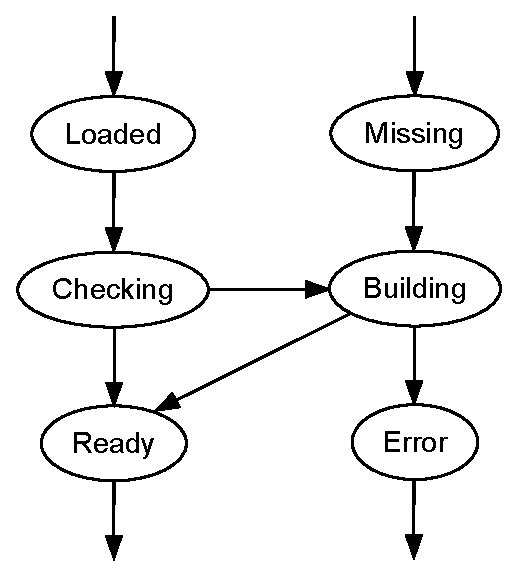
\includegraphics[scale=0.55]{states.eps}
\end{center}
\caption{Building state transitions.}
\label{fig:states}
\end{figure}

For an implementation of |build| to be correct, it must always execute enough rules to ensure all results are correct, but never execute rules that could have been safely skipped. We satisfy these constraints with the status transition diagram in Figure \ref{fig:states}. At the start of a build run all keys are either |Loaded| or |Missing|, and after calling |build| on a key, it is either |Ready| or |Error|. We use |Checking| for keys that are being checked to see if they can be skipped, and |Building| for rules that are currently being built. If a key is |Missing| and is required we have no choice but to start |Building| it. After |Building| a key, the action will either complete successfully making the result |Ready|, or fail producing an |Error|.

Most of the complexity of |build| comes from the |Checking| state, which is necessary to support unchanging results (\S\ref{sec:unchanging_results}). When checking a key there are two possibilities -- either the check succeeds and the result is |Ready|, or the check fails and we start |Building| it. We first check the stored result using |validStored|, failing the check if the result is no longer valid. We then |build| each dependency in order, and fail the check if any dependency is |Error|, or has changed since we last built this key. If all dependencies are checked successfully, we transition to |Ready|, without running the rule.

To support unchanging results, it is necessary to build dependencies \textit{before} running the rule requiring them. However, if the build system has been modified, and the rule no longer requires its previous dependencies, the dependencies may be built but not used. As a consequence, even if a key ends up in the |Error| state, the build may still complete successfully. To reduce the possibility of building many redundant keys we always check the dependencies of a rule in the order they were required, ensuring that if the rules are deterministic and have not been modified then all executed rules will be used.

\subsubsection{Efficiency}
\label{sec:parallelism}

When implementing |build| there are two separate efficiency goals. If no rules need to be run (a common case), |build| should strive for low overhead, as the time taken by |build| is likely to be a significant proportion of the total time. If rules do need running, |build| should start the rules as early as possible, to maximise parallelism. In order to expose parallelism we make |build| take a set of keys, and store |depends| as \h{type}|[[Key]]| instead of just \h{type}|[Key]| -- where each item comes from one call to |apply|.

In some ways the goals of low overhead and high parallelism are in conflict -- the first is best served by being single threaded (avoiding locks and thread contention), while the second suggests spawning many threads whenever we encounter a set of activities that could potentially be run in parallel. Our solution is to use a thread pool for running rules, a single lock to protect the state (no fine-grained locking) and a mutex for each |Checking|/|Building| state to allow other threads to wait for a result to become available. The |build| function takes the lock and, on a single thread, performs as many transitions as it can without waiting on a mutex or running any rules. Any waiting is performed after the state lock has been released, and any rules are run by adding them to a thread pool and waiting for the result. By using a thread pool we obtain high levels of parallelism, and by having a single state lock we can perform a build requiring no rules to be run with no thread contention.

Our thread pool obeys the |shakeThreads| setting (Figure \ref{fig:shake_core}), ensuring no more than a given maximum number of rules run in parallel. The thread pool is based around a pool of workers. If a new task is added to the pool, and less than |shakeThreads| workers are active, a new thread is spawned, otherwise it is queued until a worker completes. When a rule is blocked in |build|, waiting for dependencies to become available, we notify the thread pool to temporarily spawn another worker, ensuring maximum parallelism.

In order to reduce contention between processes, we run tasks added to the thread pool in a \textit{random} order. Often different build rules require different resources -- for example a compiler uses a lot of CPU while a linker does a lot of disk access. Running tasks in a deterministic order has the potential to always run all compilers followed by all linkers, resulting in lots of resource contention between different processes. A random ordering avoids the worst case scenario, and gives a noticeable speedup -- up to 20\% for some real build systems.


\section{User Tools}
\label{sec:tools}

In this section we describe three features that have been built on top of Shake -- a dependency checking tool to ensure the build system is correct, a profiling tool to determine what took most time and an analysis tool to query the build dependencies.

\subsection{Dependency checking}
\label{sec:lint}

Build systems using the theory from \S\ref{sec:theory} obtain dependencies using the |Depends| constructor, and cannot use a dependency without explicitly requesting it. However, practical build systems must integrate with IO (\S\ref{sec:user_view}), where dependencies are not always explicit. One rule can store some IO state (e.g. create a file), and another rule can use that state (e.g. read the file) without a tracked dependency, leading to inconsistent builds. We have identified three requirements Shake build systems must follow:

\paragraph{Requirement 1} If an IO action makes use of some IO state, then the rule must depend on that IO state. As an example, if a rule runs the copy command @cp from to@, then the rule must depend on @from@. In practice, we weaken this requirement in two ways. Firstly, we allow modification times as a proxy for the contents of a file, which is safe assuming any changes to a file result in changes to its modification time. Secondly, we only track file system changes within a specified directory (the users project), allowing the rule calling @cp@ to omit the dependency on the @cp@ executable, which is rarely of interest.

\paragraph{Requirement 2} If an IO action makes use of some IO state that is modified by the build system, then the rule must depend on that IO state \textit{before} performing the IO action. As an example, if a rule runs @cp from to@, and @from@ is generated by the build system, then the dependency on @from@ must be given before running @cp@. Looking at the build system in \S\ref{sec:c_example}, this build system first calls \prog{gcc} on the source files, then calls |need|, ensuring the header files are all dependencies (requirement 1 is satisfied). However, if we generate one of the header files, requirement 2 is violated because the |need| call comes after the first use -- we show how to solve this problem in \S\ref{sec:transitive}.

\paragraph{Requirement 3} After some IO state becomes a dependency it must not change for the rest of the build run. As a result, there cannot be two separate rules that modify the same file. Similarly, after |getDirectoryFiles| is called (\S\ref{sec:directory_rule}) the build system cannot create new files matching the pattern.

\smallskip\smallskip
\noindent Requirement 3 is simple to check -- after building we run the function |validStored| on all |Ready| results in the database (\S\ref{sec:parallelism}). We have implemented this feature as an option to Shake.

To check requirements 1 and 2 requires knowing which IO state is used by an IO action. For simple IO actions (e.g. |readFile|) it is easy to determine which IO state will be used, but these simple actions can usually be wrapped to provide versions which are safe by construction (e.g. |readFile'|, \S\ref{sec:derived}). For more complex IO actions, in particular the |system'| command, determining the dependencies in advance is impossible to do in a general way. The only practical approach is to \textit{trace} which IO state is used, using a system tracing mechanism (such as @strace@). File system tracing (such as @inotify@ or checking file last-access times) can provide an approximation of which IO state is used, but cannot determine if the existence of a file is tested.

The challenge when tracing IO state is cross-platform portability. Our first attempt was based around file last-access times, but on modern versions of Windows access times are turned off by default (but can be turned back on by an administrator), only accurate to one second (solvable by adding a one second delay after each IO action), and buffered for up to one hour (no feasible solution). There are no cross-platform tracing libraries, but other build systems which rely on tracing have been able to hook system libraries on Windows \cite{tup}, requiring 2000 lines of C code (more than the total size of Shake). We believe their approach could be reused in Shake, but licensing restrictions prevent us from reusing their code directly.

\subsection{Profiling}
\label{sec:profiling}

Shake records two separate pieces of profiling information.

\paragraph{Rule execution times} When running a rule we record the execution time, excluding any time building its dependencies. Execution times can be combined from different build runs, allowing us to estimate the total build time, ignoring parallelism.

\paragraph{Traced IO actions} Most time consuming rules invoke IO actions, typically system commands. To track these actions, we provide a trace function:

\begin{code}
traced :: String -> IO alpha -> Action alpha
\end{code}

\noindent All actions run by |traced| are recorded along with a human readable message (the first argument), the key being built, and the start and end times. We automatically call |traced| when running system commands. If we examine traced actions from a single run, we can determine how many traced actions were executing at each point in time -- allowing us to produce a parallelism graph as shown in Figure \ref{fig:profile}.

\smallskip\smallskip

We have built profiling support into the core of Shake. Since running a rule is likely to take some time (most rules will be spawning system processes), the overhead of recording profiling information is negligible. In previous versions of Shake we only recorded profiling information when explicitly asked, but found that users often wanted to profile the build run that had just finished -- always recording profile information makes that possible.

\subsection{Analysis}
\label{sec:analysis}

The Shake database records the dependencies of each key, allowing a full dependency graph to be produced after the rules have been run. However, for any project of moderate size, a picture of the full dependency graph is rarely comprehensible -- although with judicious filtering it is possible to produce something useful (see Figure~\ref{fig:analysis} for an example). There has been some work on visualising large build systems, for example by \citet{adams:maintaining_build_systems}, but we have not yet tried applying it to Shake.

Our approach to analysing the database is to define queries which allow end users to answer specific questions about their build system. Some of the most useful queries include:

\begin{itemize}
\item Why was a particular file rebuilt? Shake shows the complete path of dependencies, including the most recently changing dependency.
\item If I modify a file, what will rebuild? Shake computes the list of rules that depend on that file, including indirect dependencies, but assuming no unchanging results (\S\ref{sec:unchanging_results}).
\item What is the most expensive file to modify? For each leaf of the graph, Shake computes all dependencies, and then uses execution times from profiling to determine which causes most rebuilding.
\item Do my dependencies follow some layering principle? Many large projects are structured into isolated layers, this separation can be validated by the build system. For example, I would not expect any files outside \ignore|Development.Shake.*| to import any modules from inside that module tree, other than |Development.Shake| itself.
\end{itemize}

\subsection{Profiling and Analysis}

\begin{figure}
\begin{center}
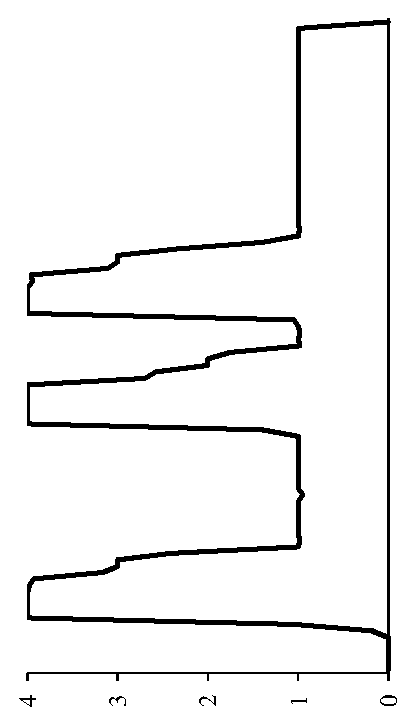
\includegraphics[scale=0.7,angle=270]{profile.eps}
\end{center}
\caption{Build parallelism.}
\label{fig:profile}
\end{figure}

\begin{figure}
\begin{center}
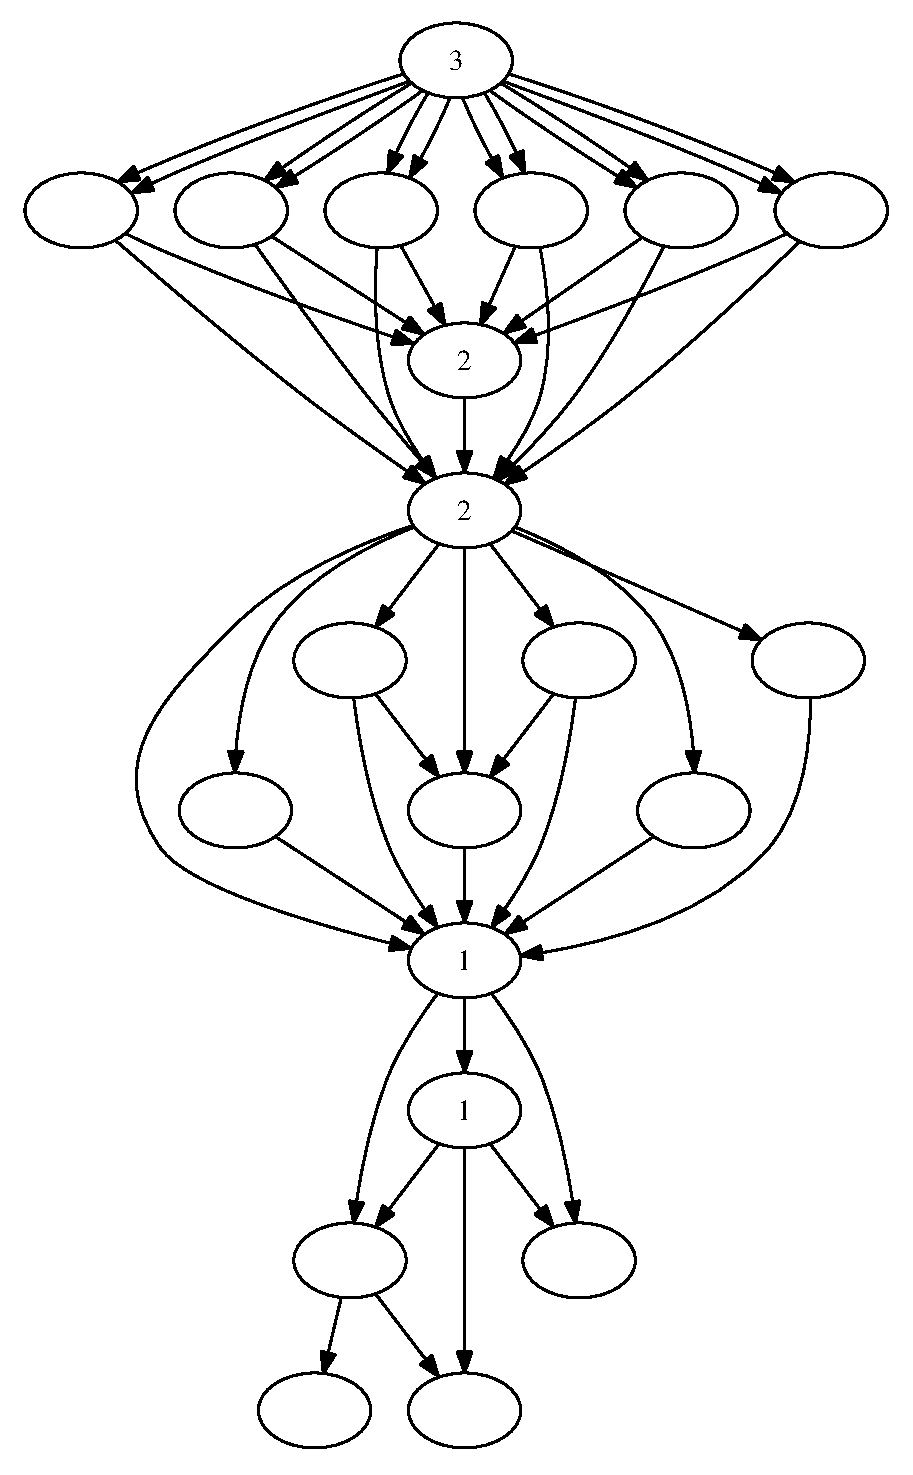
\includegraphics[scale=0.41]{layout.eps}
\end{center}
\caption{Dependency graph.}
\label{fig:analysis}
\end{figure}

% FINAL NUMBERS
% GHC full = 7.688
% GHC zero = 0.532
% Shake full -j1 = 11.828 (of which 11.702 is system commands)
% Shake full -j4 = 7.414 (of which 12.906 is system commands)
% Shake zero = 0.101 (of which 0.06 is ghc-pkg, 75% of the rest is writing the db)

As an example of the profiling and analysis tools in practice, see Figures \ref{fig:profile} and \ref{fig:analysis}. Both these diagrams are produced by building the Shake library and test harness, a 24 module Haskell program, from scratch with a maximum of four processors. The entire process takes 7.41 seconds, but spends 12.91 seconds executing rules, giving a parallel speed up of 1.7 times. Executing the build system with one processor takes 11.83 seconds -- the reduced rule execution time is likely due to reduced disk contention.

Figure \ref{fig:profile} shows the number of traced system commands executing at any point during the build. We see a start up period where zero commands are running and the build system is computing dependencies, followed by three spikes of using four processors, followed by a tail of using one processor.

The dependency graph in Figure \ref{fig:analysis} shows the dependencies of the \file{.hi} files, after hiding three utility modules which are leaves in the dependency graph (they add lots of lines, obscuring the underlying structure). It is clear the build proceeds in three stages, with bottle-neck dependencies marked 1, 2 and 3. These three bottlenecks  account for the three periods of one processor usage. The final tail of one processor includes both compilation of the main module (which profiling tells us takes 0.23 seconds) and linking (which takes 1.54 seconds).

This example shows how Shake's profiling and analysis reports can be used to improve build performance. If the bottleneck modules could be split up, or if their compilation time was reduced, the overall build time would decrease. In practice, we have found that for large build systems, where Shake is building multiple targets, parallelism usually stays at the maximum (or fractionally below it) for most of the build.

\subsubsection{Comparison to @ghc --make@ and @make@}
\label{sec:profiling_comparison}

\begin{figure}
\begin{tabular*}{\columnwidth}{@@{\extracolsep{\fill}}lrrrr@@{\extracolsep{0cm}}}
 & \prog{ghc} & Shake-1 & Shake-2 & \make{} \\
Automatic dependencies & Yes & Yes & Yes & No \\
Tracks GHC installation & Yes & Yes & No & No \\
Build on 1 thread & 7.69 & 11.83 & 11.77 & 11.75 \\
Build on 4 threads & 7.69 & 7.41 & 7.34 & 7.32 \\
No rebuilding & 0.54 & 0.10 & 0.04 & 0.02 \\
\end{tabular*}
\\

All times are in seconds. Shake-1 includes a call to @ghc-pkg list@ to track dependencies on GHC package versions, while Shake-2 assumes the GHC installation does not change.
\caption{Build time comparisons.}
\label{fig:timings}
\end{figure}

Building the same project with the GHC compilation system \cite{ghc7_2}, namely \prog{ghc --make}, takes 7.69 seconds, compared to Shake with 11.83 seconds on one processor and 7.41 seconds on four processors, see Figure \ref{fig:timings}. The reason GHC is quicker on one processor is that GHC keeps all interface information and package database information in memory, whereas running separate \prog{ghc -c} compilation commands requires reloading this information each time. However, Shake is able to use parallelism to improve the build time, while GHC cannot.

To run the build system when nothing needs compiling, GHC takes 0.54 seconds and Shake takes 0.10 seconds. Of the 0.10 seconds required by Shake, 0.06 seconds are spent checking if the GHC installation has changed (running @ghc-pkg list@) -- if the GHC installation is assumed to be constant Shake requires only 0.04 seconds. Shake is faster because it reads in one file (the database) then quickly checks |validStored| on a small number of files. GHC must query at least the same file information, but also has to construct a dependency graph, aggregating information from many files. Of the 0.04 seconds taken by Shake, 0.03 seconds are spent writing to the database -- we suspect effort spent improving the binary serialisation would reduce this overhead.

We can build the same project using \make{}, generating dependency information with \prog{ghc -M}. Unlike Shake and \prog{ghc --make}, the end user is required to regenerate \make{} rules whenever the dependencies change, and to clean the build whenever the GHC installation changes. Allowing \make{} to cope with these changes would be significantly harder, and would slow \make{} down by at least 0.12 seconds (@ghc-pkg@ and @ghc -M@ take 0.06 seconds each). In all tests, the \make{} solution is about 0.08 seconds faster than Shake, or 0.02 seconds faster if Shake avoids tracking the GHC installation. The consistency in the parallel speedup between \make{} and Shake suggests both systems are able to extract the maximum parallelism in this example.

% Compared to something like gcc, which is always invoked in single mode, we do better.
% For something like C# we don't have a choice and always run it in --make mode.


\section{Evaluation}
\label{sec:evaluation}

% Our build system has a maximum of 20 levels deep of |apply| calls from the top-level |action| statement, but 80\% of build rules are between 3 and 7 steps deep.

% [(0,2127),(1,22651),(2,190623),(3,64795),(4,15666),(5,22732),(6,10583),(7,11801),(8,5658),(9,5035),(10,3144),(11,2500),(12,974),(13,605),(14,251),(15,230),(16,73),(17,25),(18,25),(19,6),(20,1)]

At Standard Chartered we have been using build systems based on Shake for the last three years. Before Shake we used \make{}, but \make{} was a poor fit for our project, primarily due to a large number of generated files. In common with many large projects, we were forced to split our build system into several phases, where one phase generated some files and \make{} rules which were then used by a subsequent phase. Before we switched to Shake, we had over 10,000 lines of \make{} rules which were brittle and hard to extend. Our initial Shake based system was under 1,000 lines and compiled our project twice as fast -- primarily due to better parallelism from removing phases, random execution order of dependencies (\S\ref{sec:parallelism}) and faster scanning for dependencies (\S\ref{sec:transitive}).

Our Shake based build system has been an unqualified success -- while the complexity of our project has increased (more files, more compilers, more generators and more platforms), the build system has coped well. The first version of our Shake build system was under 1000 lines and matched everything the \make{} system did. Shake has been able to express all the dependencies correctly and directly, resulting in a robust build system.

From experience implementing several build systems using Shake we have learnt a number of lessons -- both about best practices for structuring build systems, and how Shake can be used to deal with the complexities of real software. In this section we share some of those lessons.

\subsection{Command Line Interface}
\label{sec:command_line}

While a build system can simply call |shake|, most systems add some command line handling, such as options to control parallelism and verbosity (see |ShakeOptions| in Figure \ref{fig:shake_core}). One common feature is a @clean@ command, to delete all build results. Using Shake we could query the database to find all build results and delete them. Alternatively, deleting the database will cause a full rebuild. However, we have found the most convenient solution is to create all build objects in a directory named \file{.make}, and perform a @clean@ by deleting that directory.

Using \make{}, you can specify build targets on the command line. We have implemented an enhanced version of this feature, allowing both individual files and sets of files to be enabled/disabled. As an example, a user may write @mk !DOCS@ to disable building documentation, or @mk index.html@ to build only \file{index.html}. We control these targets by passing a modified version of |want| to the functions specifying rules, which consults the command line arguments:

\begin{code}
documentation :: (String -> [FilePath] -> Rules()) -> Rules ()
documentation wants = do
    wants "DOCS" ["index.html"]
    "index.html" *> \out -> ellipses
\end{code}

\subsection{Build rules that change}
\label{sec:changing_rules}

Throughout this paper, we assume \textit{the build rules do not change}, merely the dependencies of the rules, but that is not true in practice. We use three techniques to minimise the impact of build rule changes:

\paragraph{Use configuration files} Most build information, such as which files a C file includes, can be computed from source files. Where such information is not available, such as which C files should be linked together to form an executable, we use configuration files to provide the information. The rule for linking can use these configuration files, which can be properly tracked. By moving any regularly changing configuration into separate files we significantly reduce the number of build system changes.

\paragraph{Depend on the build source} We should rerun a build rule if its action has changed. Lacking equality for functions, one approach is to depend on the build system source in each of the rules, then if \textit{any} actions change, \textit{everything} will rebuild. While this option is safe, it causes a significant number of redundant rebuilds. As a restricted version of this technique, for a generated file we often include a dependency on the generator source and use |writeFileChanged| (\S\ref{sec:derived}). If the generator changes it will rerun, but typically only a few generated files will change, so little is rebuilt.

\paragraph{Use a version number} There is a field named |shakeVersion| in the |ShakeOptions| record from Figure \ref{fig:shake_core}. If the build system changes in a significant and incompatible way, we increment this field to force a full rebuild. This option is a last resort, but ensures end users do not need to be aware when the build system changes, and are never required to explicitly clean their build after changes.

\subsection{Multiple Outputs}
\label{sec:multiple_outputs}

Some programs, such as the Haskell compiler \prog{ghc} \cite{ghc7_2}, can produce two outputs with one command -- compiling \file{Foo.hs} produces both \file{Foo.o} and \file{Foo.hi}. As a first approximation, the \file{.o} file depends on the entire contents of the source file, while the \file{.hi} file depends only on the type signatures. A single \prog{ghc} invocation needs to do all the work to produce both, but often the \file{.hi} file will be left unchanged. Unfortunately, many build systems (including \make{}) do not handle multiple outputs well.

In Shake, it is usually possible to describe multiple outputs in terms of single outputs -- in this example we can claim that \file{Foo.hi} depends on \file{Foo.o} with no action and \file{Foo.o} depends on \file{Foo.hs} by running \prog{ghc}. Thanks to support for unchanging files (\S\ref{sec:unchanging_results}), if the \file{.hi} file does not change then its dependencies will not be rebuilt. However, this formulation has two problems:

\begin{itemize}
\item If \file{Foo.hi} is deleted \textit{without} also deleting \file{Foo.o}, then \file{Foo.hi} will not be rebuilt by running the \file{.hi} rule, and the build system will raise an error.
\item If \prog{ghc} updates \file{Foo.hi}, but manages to determine it does not need to update \file{Foo.o}, then \file{Foo.hi} will not be marked as dirty and the build will be incorrect.
\end{itemize}

Despite these limitations, a fake dependency is often sufficient in practice, provided we can assume \file{Foo.hi} is not updated independently of \file{Foo.o}. However, consider a command that reads \file{numbers.txt} containing lines of numbers, and produces \file{even.txt} and \file{odd.txt} -- each containing only the even or odd numbers -- but does not update an output file that does not change. In this situation there is no fake dependency that adequately captures the real dependency.

\begin{figure}
\begin{code}
data Files = Files [FilePath]
data FileTimes = FileTimes [ClockTime]

instance Rule Files FileTimes where
    validStored (Files xs) (FileTimes ys) = do
        times <- mapM getFileTime xs
        return $ map Just ys == times

multipleOutputs = do
    rule $ \(Files xs) ->
        if xs /= ["even.txt","odd.txt"] then Nothing else Just $ do
            need ["numbers.txt"]
            system' "number-split" []
            times <- liftIO $ mapM getFileTime xs
            return $ FileTimes $ map fromJust times

    ["even.txt","odd.txt"] **> \_ -> do
        apply1 (Files ["even.txt","odd.txt"]) :: Action FileTimes
        return ()
\end{code}
\caption{Rule type to produce multiple outputs.}
\label{fig:multiple_outputs}
\end{figure}

We can accurately capture the dependencies using the code in Figure \ref{fig:multiple_outputs}, which introduces a new type of rule for actions producing multiple files. Inside |multipleOutputs|, the call to |rule| declares a rule that can build both \file{even.txt} and \file{odd.txt} with a single action. We call the \prog{number-split} program, and get the file times for the results. On the |**>| line we define two rules to produce the output files, using the standard file creation rules from Figure \ref{fig:file_rules}, whose action calls |apply1| with the list of files to create. If the build first requires \file{even.txt} then \prog{number-split} will be invoked, but a subsequent requirement for \file{odd.txt} will not rerun \prog{number-split}.

The Shake library wraps up the |Files| rule type, providing a simple interface using the |(*>>)| operator, allowing an end user to write:

\h{expr}\begin{code}
["even.txt","odd.txt"] *>> \_ -> do
    need ["numbers.txt"]
    system' "number-split" []
\end{code}

\subsection{Transitive Dependencies}
\label{sec:transitive}

In build systems, transitive dependencies are common -- where a rule depends on its children, plus their dependencies. As an example, if \file{foo.c} includes \file{bar.h}, and \file{bar.h} in turn includes \file{baz.h}, then \file{foo.c} should be recompiled if either \file{bar.h} \textit{or} \file{baz.h} changes. In \S\ref{sec:c_example} we saw a solution to C file dependencies, using \prog{gcc -MM} to find the transitive dependencies of a \file{.c} file then calling |need| on the results. This solution has two potential problems:

\begin{itemize}
\item If \file{bar.h} is included by many files, then both it and any headers it includes will be scanned many times. In most cases the overhead is small, but for some projects it can be significant.
\item If \file{bar.h} is generated by the build system, using \prog{gcc} will \textit{not} cause \file{bar.h} to be built, since the |need| call is performed \textit{after} running \prog{gcc} (violating requirement 2 from \S\ref{sec:lint}). If the file is missing \prog{gcc} will fail, if it is present a stale value will be used when finding its dependencies. For projects generating header files, using \prog{gcc -MM} to scan for headers is unworkable.
\end{itemize}

\begin{figure}
\h{do}\begin{code}
"*.c.o" *> \out -> do
    need =<< readFileLines (replaceExtension out "deps")
    system' "gcc" ["-c",dropExtension out,"-o",out]

"*.deps" *> \out -> do
    dep <- readFileLines $ replaceExtension out "dep"
    deps <- mapM (readFileLines . (++ ".deps")) dep
    writeFileLines out $ nub $ dep ++ concat deps

["*.c.dep","*.h.dep"] **> \out -> do
    src <- readFileLines $ dropExtension out
    let incs = [init y  |  x <- src
                        ,  Just y <- [stripPrefix hashInclude x]]
    writeFileLines out incs
\end{code}
\caption{Rules to express transitive dependencies for C files.}
\label{fig:transitive_dependencies}
\end{figure}

We can solve these problems by using the rule for \file{*.c.o} from Figure \ref{fig:transitive_dependencies}. We use a \file{.dep} file to store the immediate dependencies of a file, and a \file{.deps} file to store the transitive dependencies. For example, \file{foo.c.dep} contains the dependency \file{bar.h} while \file{foo.c.deps} contains both \file{bar.h} and \file{baz.h}. The three build rules we use are:

\begin{itemize}
\item The \file{*.c.o} rule depends on the associated \file{.deps} file (ensuring it is up to date) and then depends on its contents.
\item The \file{*.deps} rule takes the \file{.dep} file, and all the \file{.deps} it points at, producing the transitive dependencies of its immediate dependencies. This rule can be used to find the transitive dependencies of anything with \file{.dep} rules, for example with Haskell files it would produce the set of files required for linking (namely the transitive dependencies of the imports).
\item The \file{*.c.dep}/\file{*.h.dep} rule takes a source file and finds all one-level dependencies by scanning for lines starting with @#include@. This rule makes a number of assumptions about the structure of the C files which are not true in general. In particular, it assumes that includes are not skipped by @#ifdef@ commands, that there is no extra whitespace, and that local includes are quoted while system includes use angle brackets. These assumptions can be relaxed, but are sufficient for many projects.
\end{itemize}


\section{Related Work}
\label{sec:related_work}

Build tools can be divided into two categories -- those which target single-language projects with fixed rules (e.g. \prog{ocamlbuild}, \prog{ghc --make}, Visual Studio projects), and those which allow user specified rules (e.g. \make{} and Shake). Focusing on the second category, the defacto standard is \make{}, but there are many \make{} competitors (notably Ant, CMake, Jam, Scons and Waf). Most of these tools read a list of rules, generate a dependency graph, then execute commands while traversing that graph.

Since the number of build tools is vast, we focus on four build tools which take different approaches (Redo, Ninja, Tup and Fabricate). Interestingly, one thing all four systems have in common is that they require a database of build data, in addition to the rules and the file system. Unlike Shake, all these build systems are limited to files.

\subsection{Redo}

% https://github.com/apenwarr/redo

The Redo build system \cite{redo} has a similar dependency theory to Shake. Rules are run starting at the target. A rule may call \textsf{redo-ifchange} (similar to |need|) to ensure that this rule is repeated if any of the file arguments change. A rule can build either a specific named file, or a set of files ending with a particular extension.

While Redo has similarities to Shake, the practical implementation is significantly different. Instead of a single rule store, Redo stores each rule in a separate file, and the script language is simply shell script (allowing @#!@ to change the interpreter). The advantage of separate files is that Redo is able to depend on the actual rule used to build a result, meaning that build system changes are properly tracked. However, separating build rules makes it harder to reason about the build system, and eliminates many potential uses of abstraction \cite{jonge:build_components}. Redo does not work on Windows, and has no support for unchanging files or multiple outputs.

\subsection{Ninja}

% http://martine.github.com/ninja/manual.html

The Ninja build system \cite{ninja} is designed as a two-stage build system -- users specify their build rules in a high-level manner, which is then translated to a set of Ninja build rules. As a result, the Ninja build system is not designed to be general purpose and configuration choices are expected to be resolved by the first level. The Ninja target language supports three dependency features beyond \make{}. Firstly, a rule can depend on the list of files contained in another file, allowing additional dependencies at build time. Secondly, the command line for each rule is tracked, resulting in a rebuild if the rule itself changes. Thirdly, a rule can generate multiple outputs, which are properly tracked.

\subsection{Tup}

% http://gittup.org/tup/build_system_rules_and_algorithms.pdf

The Tup build system \cite{tup} is designed as an incremental build system. Tup has a similar dependency structure to \make{}, but a significantly different implementation. Instead of scanning all dependencies, it expects the operating system to supply a list of changed files, avoiding the overhead of checking which files have changed. For large build systems the result can be a significant speed improvement when rebuilding only a few files. We believe a similar implementation strategy could be applied to Shake.

Another difference from \make{} is the treatment of dead build results. If a rule to build \file{foo} is deleted from the rule list, then Tup automatically deletes the file \file{foo}. The problem of dead build results is serious, resulting in builds succeeding that should have failed, and that will fail as soon as a clean build is performed (to reduce this risk, we suggest an overnight build which starts from scratch). However, it is often useful to have build modes which generate skeleton files which are then modified by the user -- deleting these files would be most unwelcome. It would be easy to add support for deleting dead build results to Shake, but we choose not to.

\subsection{Fabricate}

% http://code.google.com/p/fabricate/

The key innovation in the Fabricate build system \cite{fabricate} is that dependencies do not need to be stated explicitly. A build system is a Python program, which primarily executes system commands in order. While executing the commands, Fabricate uses system tracing (strace on Linux) to record which files are accessed. In future runs, if the same system command is reached but none of the files it used have changed, the command is skipped. The resulting build systems are simple, and avoid the difficulties of correctly specifying dependencies.

There are two inherent difficulties for build systems without explicit dependencies. Firstly, the system tracing mechanisms on different platforms are varied, and on Windows are somewhat fragile (see \S\ref{sec:lint}). Secondly, parallelism cannot be inferred automatically -- Fabricate requires explicit grouping annotations to use parallelism.

\subsection{Extending Make Dependencies}
\label{sec:make_hacks}

Specifying additional dependencies while building is critical for many projects. As a result, a number of techniques have been developed to specify additional dependencies in \make{}. Most of these techniques rely on \textit{generating} some portion of the \make{} rules file, either before \make{} starts, or invoking \make{} multiple times. Taking the example from \S\ref{sec:introduction}, we can write it with \make{} as:

\ignore\begin{code}
{-"\textsf{result.tar : list.txt \$(shell cat list.txt)}"-}
    {-"\textsf{cat list.txt}"-} | {-"\textsf{xargs tar -cf result.tar}"-}
\end{code}

Here \make{} is executing commands in two distinct phases -- the first phase generates the rules file, the second runs it. In many large projects, the first phase becomes expensive or complex, resulting in specific commands such as @make depends@ to update the dependencies (as required in \S\ref{sec:profiling_comparison} and \S\ref{sec:evaluation}). Another approach is for \make{} to restart itself partway through the build, after modifying the build rules. However, multiple phases have many problems:

\begin{itemize}
\item There is no limit to the number of build phases required, especially when files are generated by the build system. Shake was originally designed after determining a particular build system required seven phases.
\item The introduction of phases breaks compositionality, requiring build system authors to globally separate rules by phase. The above rule for \file{result.tar} fails if \file{list.txt} is itself built by the build system, whereas the Shake rule in \S\ref{sec:introduction} works in all cases.
\item These approaches require generating \make{} rules as text, which is then reinterpreted by \make{}. As a result, while the Shake rule from \S\ref{sec:introduction} can handle spaces in file names, the \make{} rule cannot. Fortunately, many compilers already support generating well-formed \make{} rules for their dependencies.
\item If all phases are run every time then there is overhead due to restarting \make{}, rechecking previously checked rules and reducing parallelism opportunities. If different phases are invoked manually then the user has to be aware what has changed.
\end{itemize}

\subsection{Haskell Build Libraries}

There are a surprisingly large number of Haskell libraries implementing a dependency aware build system -- we know of ten in addition to Shake (Abba, Blueprint, Coadjute, Cake $\times$ 2, Hake, Hmk, Nemesis, OpenShake and Zoom). Of these, the two Cake libraries and OpenShake are based on an early presentation of the principles behind Shake, before the source code was available. The primary difference from the Cake libraries is that this paper allows multiple types of build rule, while the Cake libraries only allow file rules. Compared to OpenShake \cite{openshake}, we have opted to have |rule|/|apply| based on dynamic types, and then use sugared versions to regain static guarantees of type safety. In contrast, OpenShake uses type functions \cite{schrijvers:type_functions} to statically track the available rule types, making serialisation simpler (\S\ref{sec:dynamically_typed}), but complicating the rest of the library.


\section{Conclusions and Future Work}
\label{sec:conclusions}

We have presented a dependency model which allows additional dependencies to be specified \textit{after} the build system starts running rules. This additional flexibility is essential for many build systems, especially those where source files are generated by rules. We have implemented our ideas in the Haskell library Shake, producing a user-friendly interface combined with an efficient and robust implementation. We have used Shake extensively and find it much easier to use than \make{} (\S\ref{sec:evaluation}).

Functional programming is important for Shake. The theory of build systems is naturally expressed using higher-order functions, where actions are functions from dependencies to results. Moving towards a practical build system, a major consideration is the treatment of IO -- we use monads to restrict where IO can be used, while also using monads to track state in a thread-safe way. We make use of the flexible syntax of Haskell to allow Shake rules to be written with minimal syntactic overhead. Laziness is not necessary for Shake, and if ignored could cause problems, but restricting laziness is simple (\S\ref{sec:handling_errors}).

While we have optimised our build algorithms, saving the database is a noticeable bottleneck for quick builds, taking upto 75\% of the time. We suspect this step could be sped up, perhaps by switching to a different binary serialisation library. We have provided some tools on top of Shake, but improvements to the analysis feature would help Shake users, as would fully implementing dependency checking. Some users have already begun work on general purpose build rules for common types of source code, which could reduce the effort required to make use of Shake.

The \make{} tool has been ubiquitous for the last thirty years, specifying dependencies in advance and defining actions with shell scripting and a macro system. With Shake we offer more powerful dependencies, coupled with the Haskell language for defining actions. The dependencies allow more complex build systems to be specified in a more direct manner, while the use of Haskell allows abstraction and reuse. We hope these advantages are powerful enough to tempt many developers to consider Shake.

\paragraph{Acknowledgements}

Thanks to Standard Chartered, where Shake was initially developed, and to Raphael Montelatici for the name Shake. Thanks to Max Bolingbroke and Evan Laforge for many discussions about build systems. Thanks to S\"{o}nke Hahn, Evan Laforge, Roman Leshchinskiy and Raphael Montelatici for comments on drafts of this paper.


\bibliographystyle{plainnat}
\balance
\bibliography

\end{document}
